\section{Entity Relationship Model}
By receiving a set of requirements, we need to design an application. For the data behind it, we must create a database schema that provides a logical view of the data model. However, the main challenge is how to build a database for this application that meets all the requirements — in other words, how to construct a systematic database.  

In this case, we use Chen's \textbf{Entity-Relationship (ER) Model}. In this model, there are two major components: \textbf{Entities} and \textbf{Relationships}. An \textbf{Entity} is a collection of attributes that describe an object of interest, while a \textbf{Relationship} represents the association between entities (objects). There is also a third component, the \textbf{Attribute}, which is a data item describing a property of interest.  

Let us now look at the details.

\subsection{Entity}
An \textbf{Entity} is something that is distinguishable from other objects. For example, entities can be \emph{Classrooms}, \emph{Students}, etc. Entities represent things in the real world, and \textbf{Attributes} describe their properties.  

Some attributes are simple (also called \emph{atomic}), meaning they cannot be split into simpler components. Each simple attribute of an entity type holds one value. It is associated with a \textbf{value set} (or \emph{domain}), which specifies the possible values that may be assigned to that attribute for each individual entity.  

An entity is described using a set of attributes whose values distinguish one entity from another of the same type. An \textbf{Entity Set} is a collection of such entities (instances of the entity type).  

For each attribute associated with an entity set, we must identify a domain of possible values.  

To describe data in terms of a data model, we use a \textbf{schema}. For example, for a \emph{Student} entity set, we may define the schema:  

\[
\text{Students}(\text{sid: string}, \; \text{name: string}, \; \text{login: string}, \; \text{age: integer}, \; \text{gpa: real})
\]  

A good entity schema should include attributes that are meaningful, well-defined, and capable of being filled with valid values.

\subsection{E-R Diagrams}
Data modeling is typically divided into three tiers:  

1. \textbf{Semantic (High-level or Conceptual)} — provides an initial description of the data in the enterprise.  

2. \textbf{Implementation (or Record-based)} — describes how data can be organized using models such as the Relational, Network, or Hierarchical model.  

3. \textbf{Low-level (or Physical)} — specifies details such as record formats, access paths, and storage structures.  

To develop a database, we must first analyze the requirements, then design and implement the data model. The \textbf{Entity-Relationship (E-R) diagram} is often used for conceptual modeling.

For example, in Figure~1.1, the E-R diagram represents the following description:

\begin{quote}
“There is one strong entity type called \emph{Car}. It has a multivalued attribute to describe its color. It also has a composite attribute \emph{Registration}, which consists of \emph{Registration Number} and \emph{State}. Additionally, it includes several other attributes such as \emph{Make}, \emph{Model}, and \emph{Year}.”
\end{quote}

\begin{figure}[H]
  \centering
  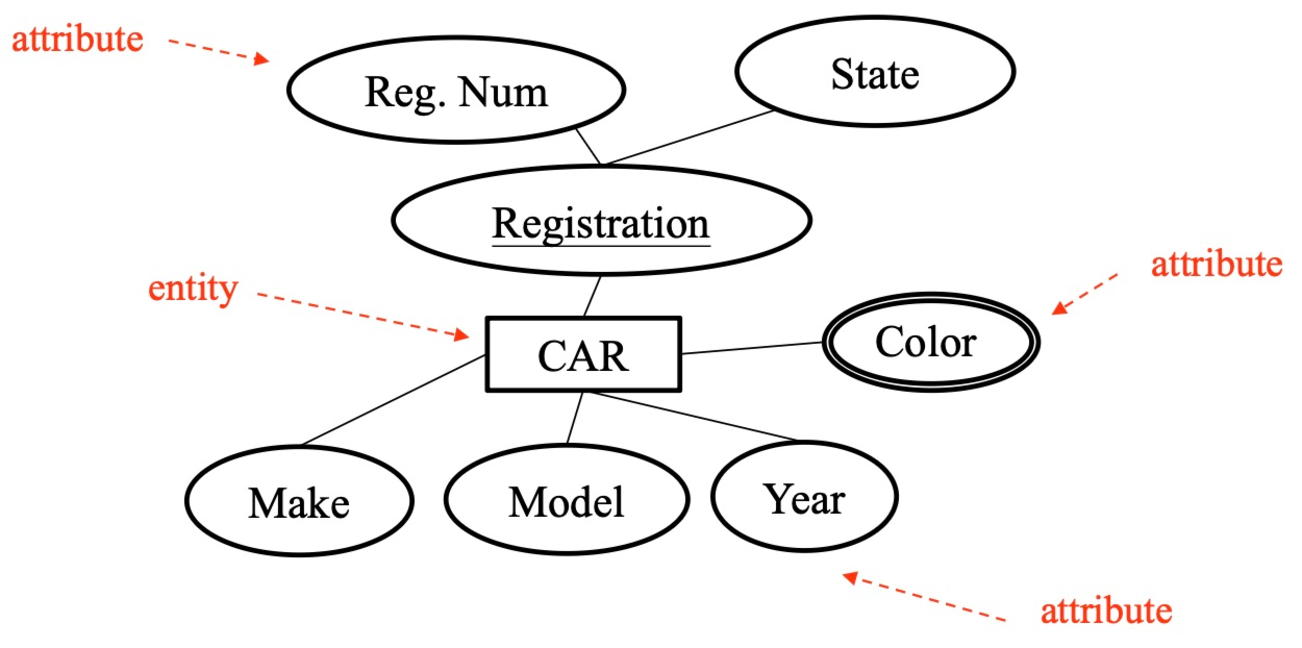
\includegraphics[width=0.6\textwidth]{Figure/ER1.pdf}
  \caption{E-R Diagram: Car entity}
\end{figure}

\subsection{Relationship}
We have discussed \textbf{Entities} and \textbf{Attributes} in the Entity–Relationship (E-R) Model. The second major component is the \textbf{Relationship}.  

A relationship can also have \textbf{descriptive attributes} (see Figure~1.2). Descriptive attributes are used to record information about the relationship itself, rather than about any of the participating entities.  

\begin{figure}[H]
  \centering
  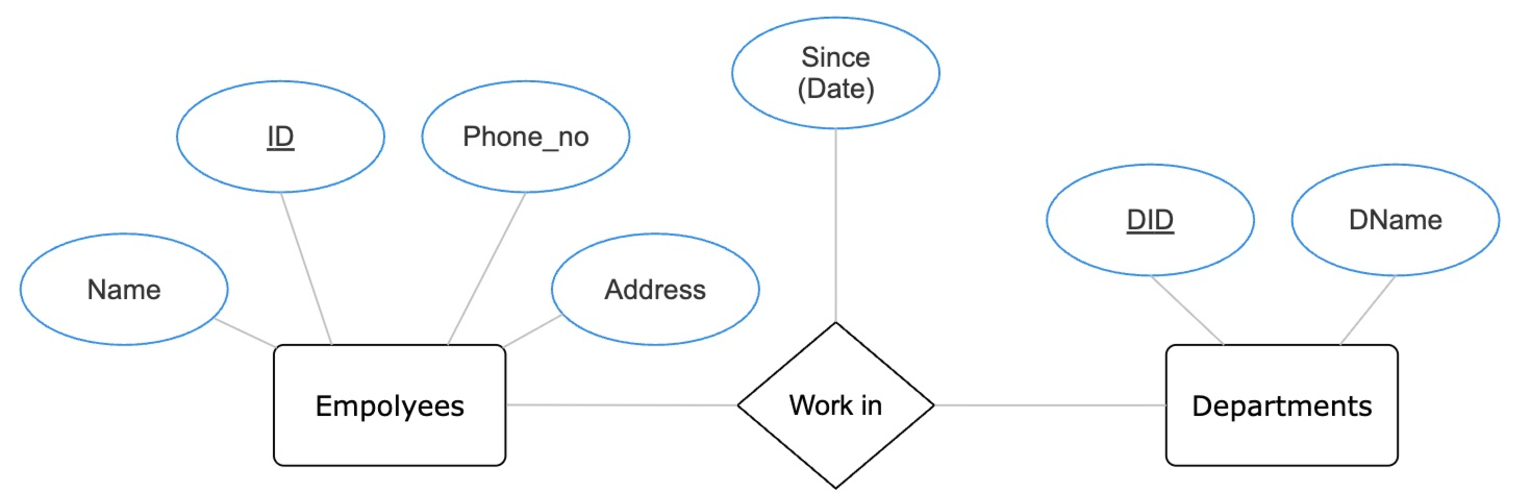
\includegraphics[width=0.6\textwidth]{Figure/ER2.pdf}
  \caption{E-R Diagram: Relationship}
\end{figure}

Relationships represent logical links between two or more entities. Any set of entities is not limited to participating in only one relationship with each other.  

An \textbf{Entity–Occurrence Diagram} shows the relationships between individual occurrences (instances) of particular entities.  

\begin{figure}[H]
  \centering
  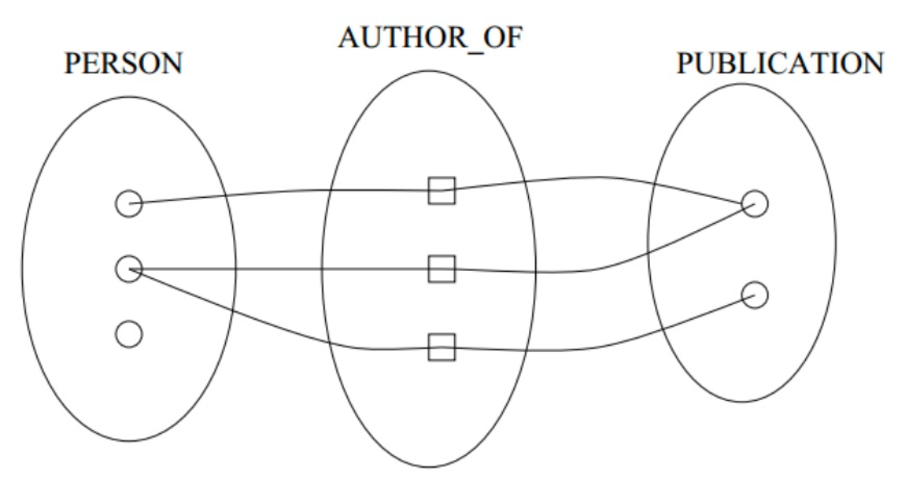
\includegraphics[width=0.6\textwidth]{Figure/ER3.pdf}
  \caption{Many-to-Many Relationship}
\end{figure}

There are three main types of relationships. To distinguish among them, we apply two types of constraints: \textbf{cardinality} and \textbf{participation}.  

\subsection{Cardinality}

The \textbf{cardinality constraint} (or \emph{cardinality ratio}) specifies the number of relationship instances an entity can participate in. The three common types are:
\begin{itemize}
  \item \textbf{1:1 (one-to-one)} — each entity instance is associated with at most one instance of another entity.
  \item \textbf{1:N (one-to-many)} — one entity instance can be associated with many instances of another entity.
  \item \textbf{M:N (many-to-many)} — multiple instances of one entity can be associated with multiple instances of another entity.
\end{itemize}

We can use standard \textbf{entity–occurrence diagrams} to visualize such relationships.

\begin{figure}[H]
  \centering
  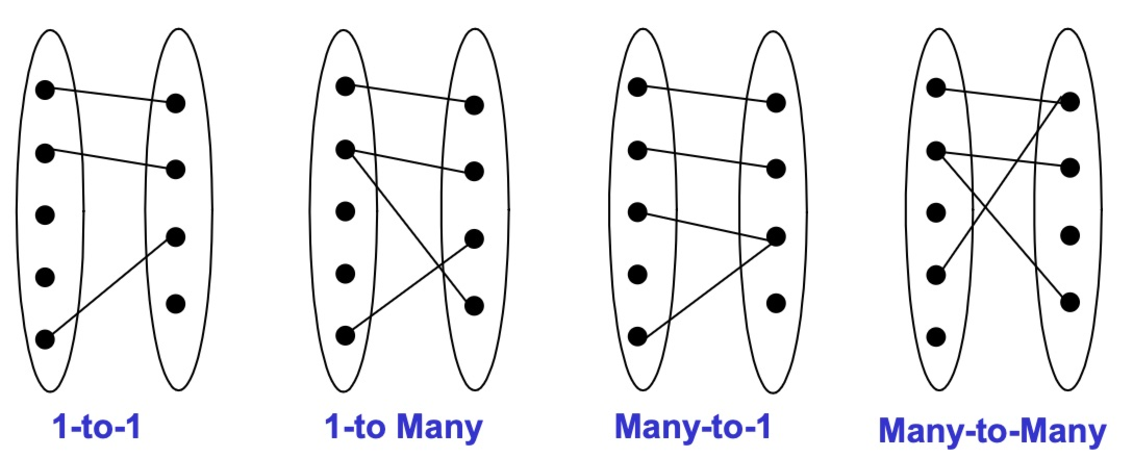
\includegraphics[width=0.6\textwidth]{Figure/EOD1.pdf}
  \caption{Standard Entity-Occurrence Diagrams}
\end{figure}

\subsubsection{One-to-Many}
One-to-many constraint from A to B: an entity in B can be associated with at most one entity in A.

To represent such relationships, we use arrows in the diagram. An arrow indicates that one entity can be uniquely associated with a relationship instance.  

For example, in the following case, each \emph{Employee} belongs to one \emph{Department}, while a \emph{Department} may have multiple employees. We use an arrow pointing from the \emph{Employee} entity set to the \emph{works\_in} relationship to represent this constraint.

\begin{figure}[H]
  \centering
  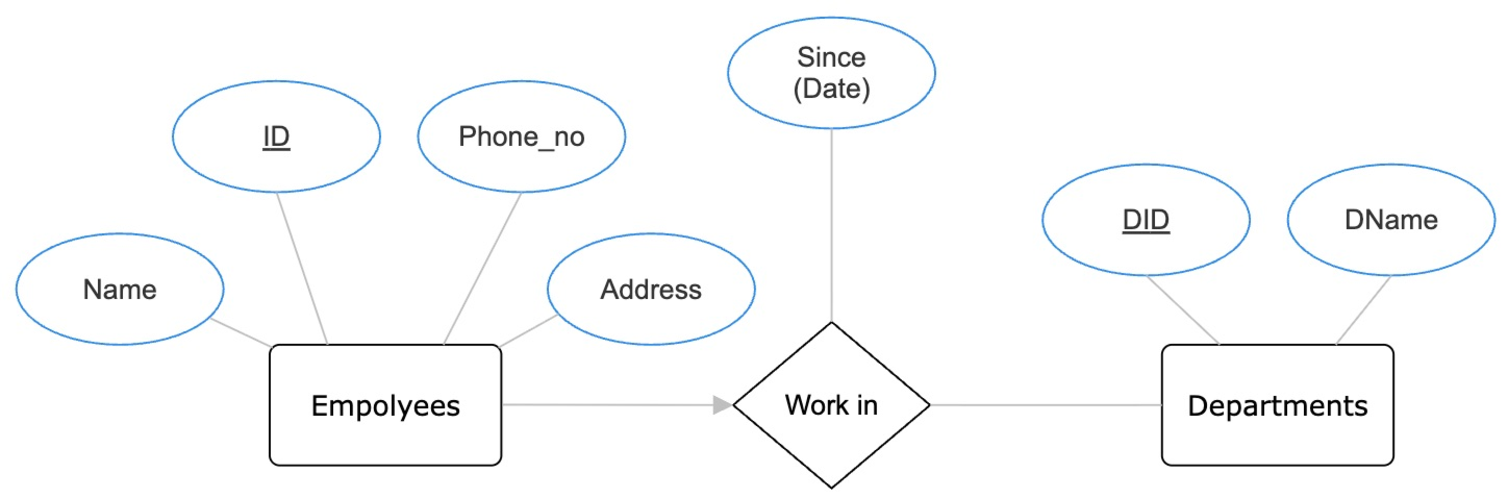
\includegraphics[width=0.6\textwidth]{Figure/ER4.pdf}
  \caption{E-R Diagram: One-to-many}
\end{figure}

\subsubsection{One-to-One}
If a relationship between \emph{A} and \emph{B} satisfies the one-to-one mapping constraint, i.e., each entity in \emph{A} is related to at most one entity in \emph{B}, and each entity in \emph{B} is related to at most one entity in \emph{A},  

we represent this relationship with two arrows, one pointing from \emph{A} to \emph{B} and one from \emph{B} to \emph{A}.

\begin{figure}[H]
  \centering
  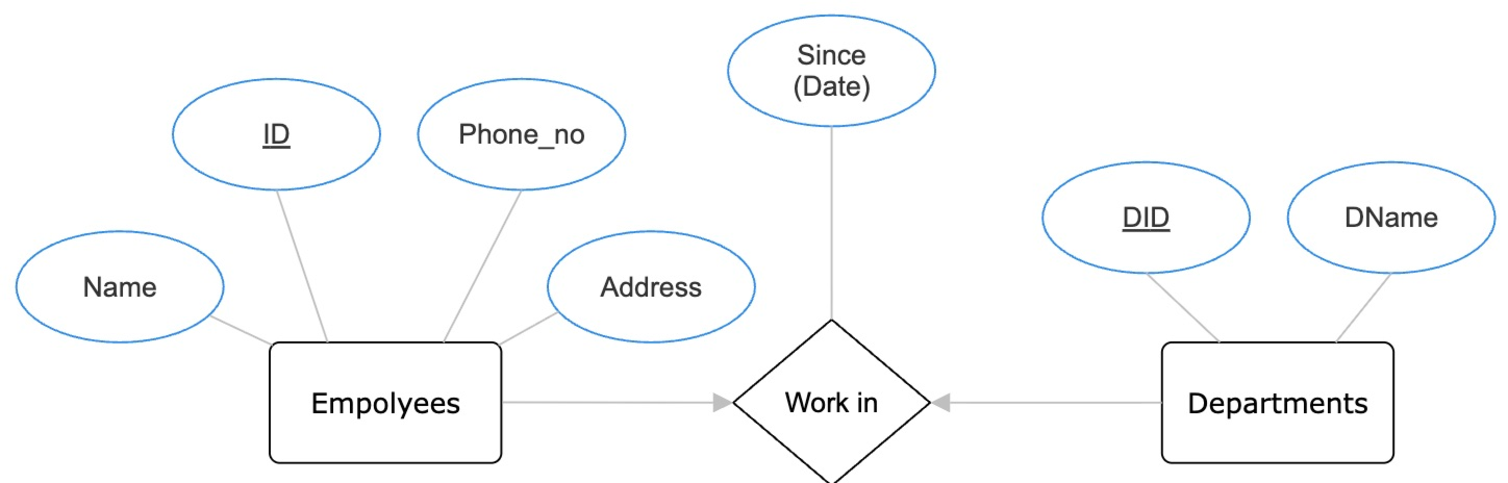
\includegraphics[width=0.6\textwidth]{Figure/ER5.pdf}
  \caption{E-R Diagram: One-to-One}
\end{figure}

\subsubsection{Many-to-Many}
If an entity in \emph{A} can be associated with any number of entities in \emph{B}, and an entity in \emph{B} can be associated with any number of entities in \emph{A}, this indicates that there is no restriction on the mapping.

\subsection{Participation}
In a one-to-one relationship, as shown in Figure~1.6, if we change the \emph{works\_in} relationship to \emph{manages}, one question arises: is there at least one manager in each department? The cardinality constraint does not provide this information. Therefore, we need \textbf{participation constraints}.

We can classify participation in relationships as follows:
\begin{itemize}
  \item \textbf{Total participation} — every entity in the entity set must participate in at least one relationship.
  \item \textbf{Partial participation} — an entity in the entity set may not participate in any relationship.
\end{itemize}

In an E-R diagram, total participation is represented by a double line, while partial participation is represented by a single line.  

\begin{figure}[H]
  \centering
  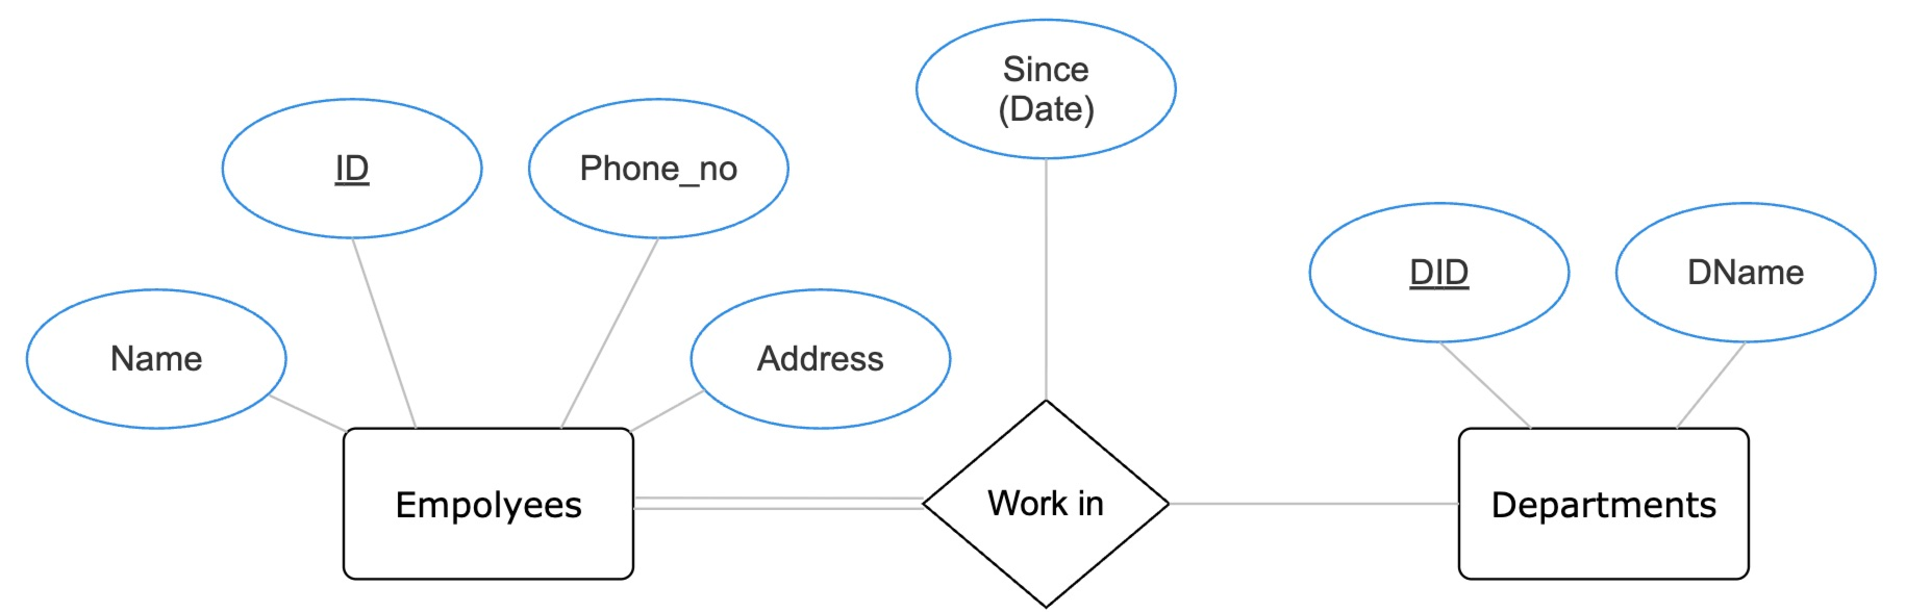
\includegraphics[width=0.6\textwidth]{Figure/ER6.pdf}
  \caption{E-R Diagram: Total Participation}
\end{figure}

As shown in Figure~1.7, this indicates that every \emph{Employee} must work for some \emph{Department}.

\subsection{Attributes}
The final component of Entity–Relationship (E-R) modeling is \textbf{Attributes}.  

Some semantics cannot be captured using simple (atomic) attributes. In such cases, we use \textbf{multivalued attributes}, which are represented by a double ellipse in an E-R diagram.  

We also have \textbf{composite attributes}. Unlike simple attributes, which are indivisible, composite attributes can be divided into smaller subparts, each representing a more basic attribute with independent meaning.  

Another type is \textbf{derived attributes}. These are attributes whose values can be derived from other attributes, rather than being stored directly. For example, a person's \emph{age} can be derived from their \emph{date of birth}. In an E-R diagram, derived attributes are represented by a dashed ellipse.
